\documentclass{article}
\usepackage{neurips_2019}

\usepackage[utf8]{inputenc} % allow utf-8 input
\usepackage[T1]{fontenc}    % use 8-bit T1 fonts
\usepackage{hyperref}       % hyperlinks
\usepackage{url}            % simple URL typesetting
\usepackage{booktabs}       % professional-quality tables
\usepackage{amsfonts}       % blackboard math symbols
\usepackage{nicefrac}       % compact symbols for 1/2, etc.
\usepackage{microtype}      % microtypography
\usepackage{graphicx}

% Useful packages
\usepackage{amsmath, amssymb, amsfonts, bm}
\usepackage{amsthm}
\usepackage{mathtools}
\usepackage[usenames, dvipsnames]{color}

\usepackage{blindtext}


\newcommand{\tk}[1]{\textcolor{red}{TK: #1}}
\newcommand{\ao}[1]{\textcolor{green}{AO: #1}}
\newcommand{\tsj}[1]{\textcolor{magenta}{TSJ: #1}}
\newcommand{\va}[1]{\textcolor{blue}{Vincent A: #1}}

\title{A New Model}

\author{
	T.S. Jayram \And Vincent Albouy  \And Tomasz Kornuta \And Ahmet S. Ozcan}

\begin{document}

\maketitle

\blindtext

\begin{figure}[ht]
	\centering
	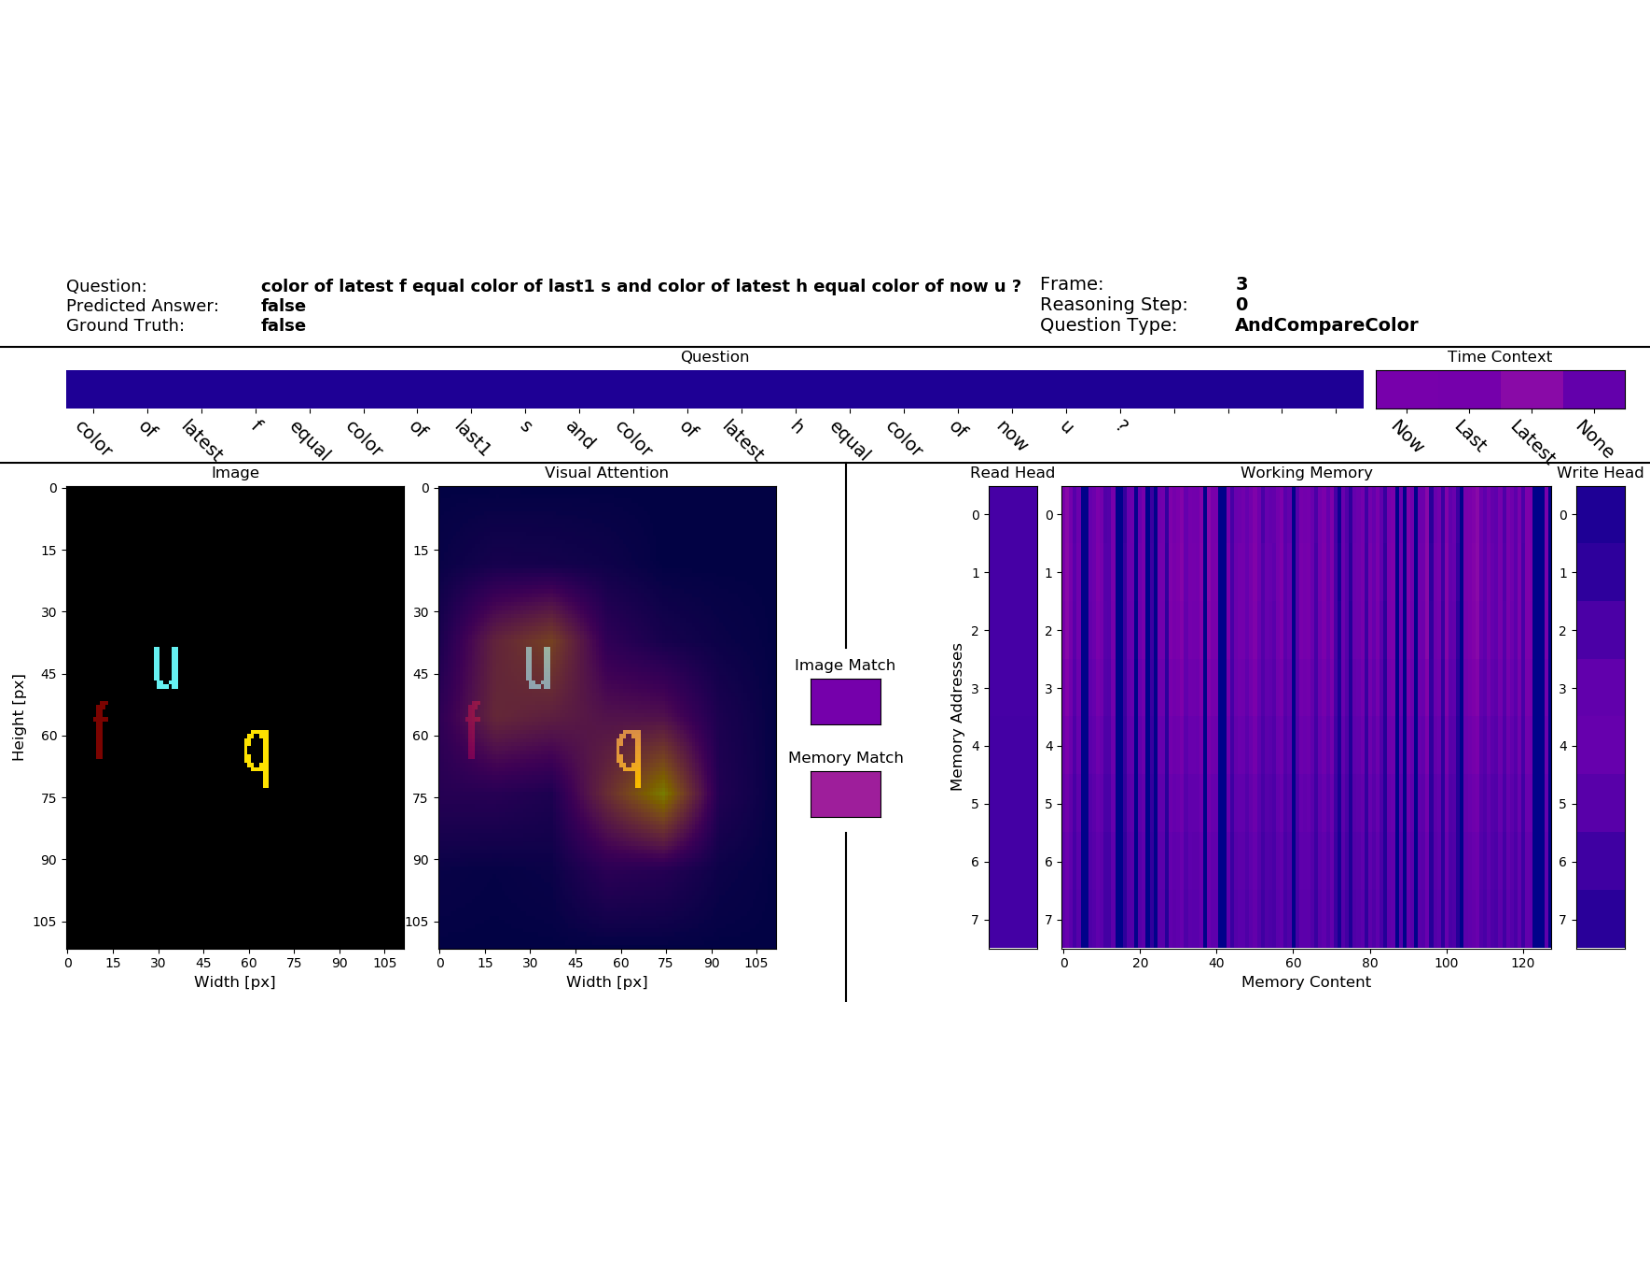
\includegraphics[width=\textwidth]{img/visualization}
	\caption{Testing}
	\label{fig:visualization}
\end{figure}

\blindmathtrue

\blindtext

\blindmathfalse

\section{VWM model}

\begin{figure}[ht]
	\centering
	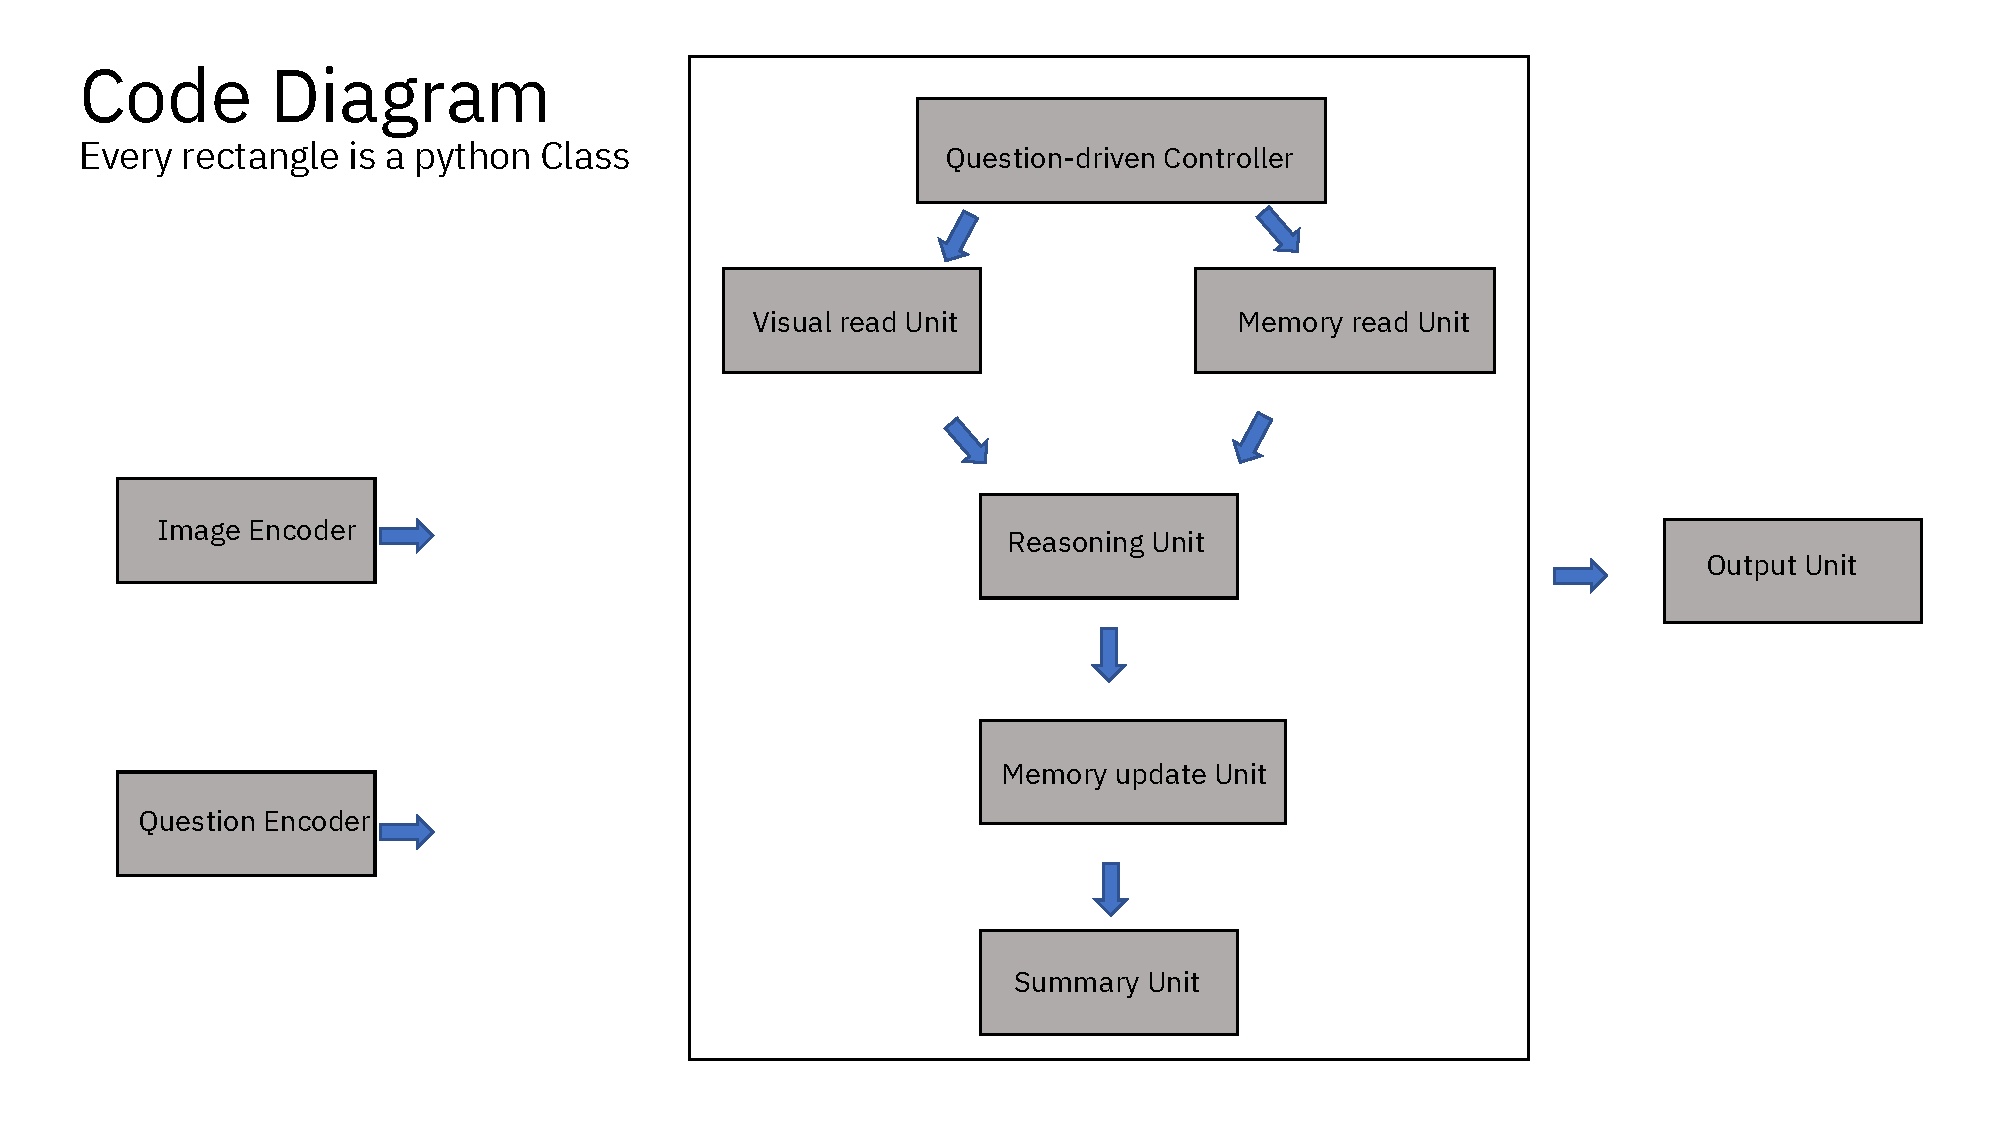
\includegraphics[width=\textwidth]{img/model}
	\caption{Testing}
	\label{fig:model}
\end{figure}



\newpage
\bibliographystyle{alpha}

\end{document}
